\begin{figure}[htbp]
\section*{ TGFB2}
\centering
\begin{subfigure}[b]{0.95\textwidth}
\centering
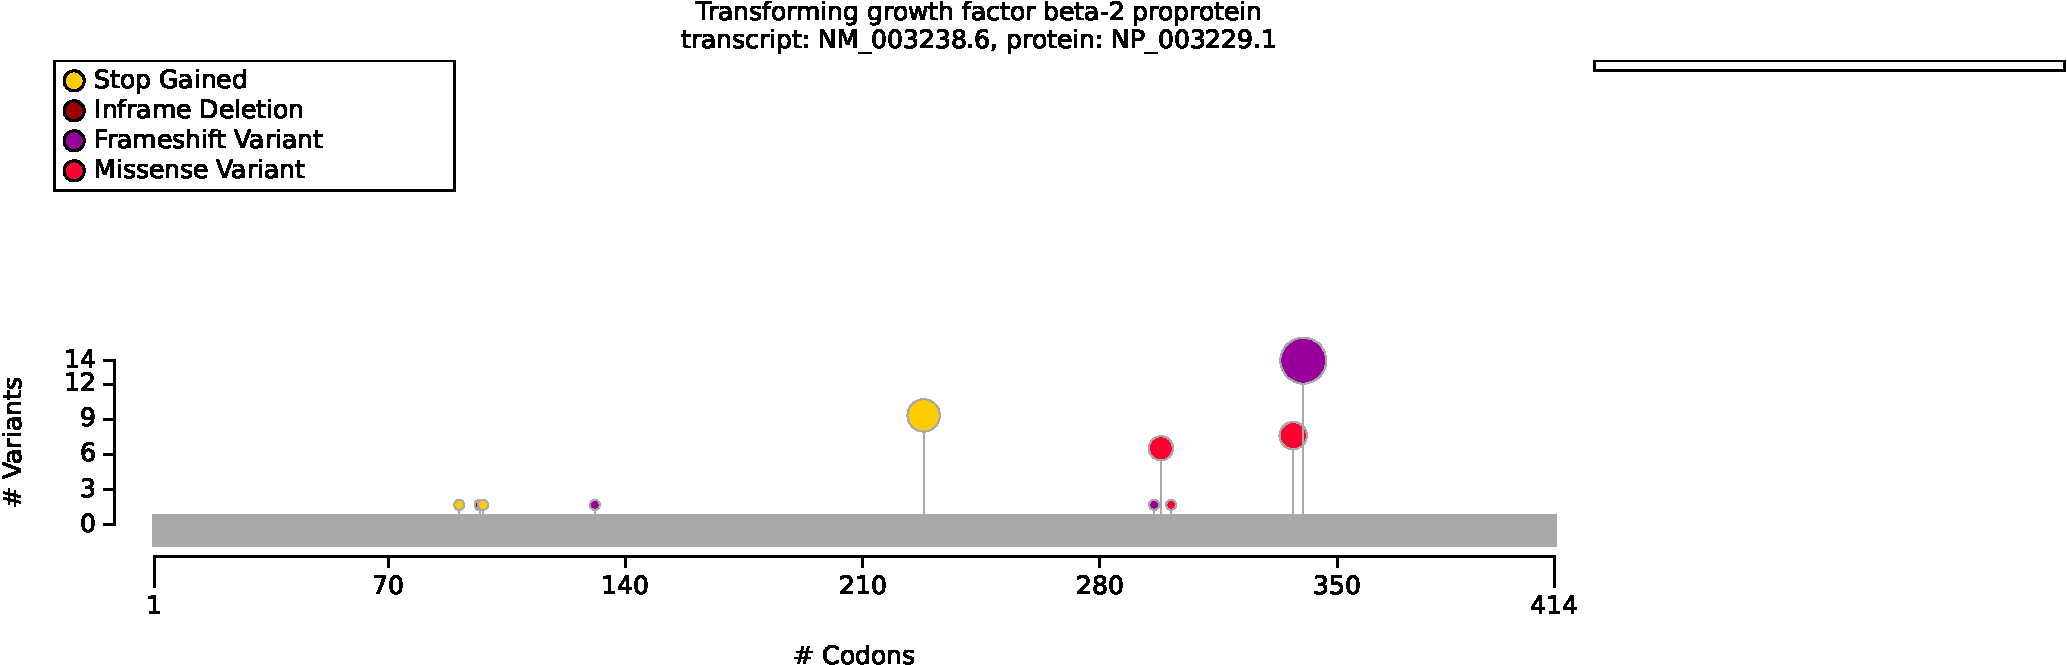
\includegraphics[width=\textwidth]{ img/TGFB2_protein_diagram.pdf} 
\captionsetup{justification=raggedright,singlelinecheck=false}
\caption{Distribution of variants in TGFB2}
\end{subfigure}

\vspace{2em}

\begin{subfigure}[b]{0.95\textwidth}
\centering
\resizebox{\textwidth}{!}{
\begin{tabular}{llllrr}
\toprule
Genotype (A) & Genotype (B) & total tests performed & significant results\\
\midrule
missense & other & 31 & 0\\
FEMALE & MALE & 31 & 0\\
\bottomrule
\end{tabular}
}
\captionsetup{justification=raggedright,singlelinecheck=false}
\caption{Fisher Exact Test performed to compare HPO annotation frequency with respect to genotypes. }
\end{subfigure}

\vspace{2em}

\caption{ The cohort comprised 36 individuals (10 females, 26 males). 1 of these individuals were reported to be deceased. A total of 68 HPO terms were used to annotate the cohort. Disease diagnosis: Loeys-Dietz syndrome 4 (OMIM:614816). No significant association found. A total of 36 unique variant alleles were found in \textit{TGFB2} (transcript: \texttt{NM\_003238.6}, protein id: \texttt{NP\_003229.1}).}
\end{figure}
